\documentclass[12pt,a4paper]{article}
\usepackage[T1]{fontenc}
\usepackage{libertinus}

\usepackage{hyperref}

\usepackage{amsmath}
\usepackage{unicode-math}

\usepackage{listings}

\usepackage{tikz}
\usetikzlibrary{shapes.geometric}


\lstdefinestyle{mystyle}{
	numbers=left,
	basicstyle=\ttfamily,
	frame=single}

\lstset{style=mystyle}

\begin{document}

\section{Python listing}
	
From directlua -> \directlua{tex.print("\\LaTeX")}

\begin{lstlisting}
import os
import random
from itertools import groupby

import matplotlib.pyplot as plt

random.seed(os.urandom(128))

ball_move_Left = -1
ball_move_Right = 1


def oneBall(stages: int) -> int:
    return sum([random.choice([ball_move_Left, ball_move_Right]) for _ in range(stages)])


def galton(stages: int, n_balls: int):
    all_results = sorted([oneBall(stages) for _ in range(n_balls)])
    position = []
    counter = []
    for k, g in groupby(all_results):
        position.append(k)
        counter.append(len(list(g)))

    fig, ax = plt.subplots()
    ax.bar(position, counter)

    ax.set_xlim([-stages, stages])
    ax.set_xlabel("Position")
    ax.set_ylabel("Times")

    fig.show()


galton(100, 5000)
\end{lstlisting}

\section{Draw staff}

\begin{center}
	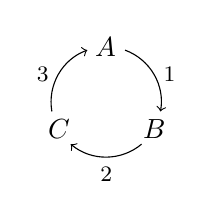
\begin{tikzpicture}[->,scale=.7]
		\node (i) at (90:1cm) {$A$};
		\node (j) at (-30:1cm) {$B$};
		\node (k) at (210:1cm) {$C$};
		\draw (70:1cm) arc (70:-10:1cm) node[midway, right] {{\footnotesize 1}};
		\draw (-50:1cm) arc (-50:-130:1cm) node[midway, below] {{\footnotesize 2}};
		\draw (190:1cm) arc (190:110:1cm) node[midway, left] {{\footnotesize 3}};
	\end{tikzpicture}
\end{center}

\section{PDF calculator}

Works in Firefox.\\

\begin{Form}
	\noindent%
	\TextField[name=a]{a:} \\ \\
	\TextField[name=b]{b:} \\ \\
	\TextField[name=c]{c:} \\ \\
	\noindent%
	$\sum = $ \TextField[name=AvgStat, calculate={
		event.value = (this.getField("a").value + this.getField("b").value + this.getField("c").value);
	}, readonly, value=0]{}
\end{Form}

\end{document}
